\documentclass[a4paper,capchap,espacoduplo,normaltoc]{abntepusp} % Mude "abntepusp" para "abntepusp-en" para Ingl�s.

%\usepackage[bookmarks,pdftex,a4paper,colorlinks=true,citecolor=black,urlcolor=blue,linkcolor=black,pdfpagemode=None]{hyperref}
\usepackage[bookmarks,colorlinks=true,citecolor=black,urlcolor=blue,linkcolor=black,pdfpagemode=UseNone]{hyperref}
\usepackage[centertags]{amsmath}
\usepackage{amsfonts}
\usepackage{amssymb}
\usepackage{amsthm}
\usepackage[T1]{fontenc}
\usepackage[latin1]{inputenc}
\usepackage[brazil]{babel} % Mude "brazil" para "english" para Ingl�s.
\usepackage[alf,abnt-repeated-author-omit=yes]{abntcite}
%\usepackage[alf,abnt-repeated-author-omit=yes]{abntex2cite}
\usepackage{url}
%\usepackage{winfonts}
\usepackage{txfonts}
\usepackage[ddmmyyyy]{datetime}
\usepackage{graphicx}

%\fontfamily{arial}\selectfont
%\renewcommand{\rmdefault}{arial}

% Comando �til
\newcommand{\TODO}[1]{~~\textcolor{red} {\textbf{TODO: #1}}}

% Math -------------------------------------------------------------------
\newtheorem{theorem}{Teorema}{\bfseries}{\itshape}
\newtheorem{lemma}{Lema}{\bfseries}{\itshape}
\newtheorem{definition}{Defini��o}{\bfseries}{\itshape}
\newtheorem{corollary}{Corol�rio}{\bfseries}{\itshape}
\newtheoremstyle{example}{\topsep}{\topsep}%
	{}%         Body font
	{}%         Indent amount (empty = no indent, \parindent = para indent)
	{\bfseries}% Thm head font
	{:}%        Punctuation after thm head
	{.5em}%     Space after thm head (\newline = linebreak)
	{\thmname{#1}\thmnumber{ #2}\thmnote{ #3}}%         Thm head spec
\theoremstyle{example}
\newtheorem{example}{Exemplo}

\sloppy

\begin{document}

% documento propriamente monogr�fico: um �nico autor
%\autorPoliI{Nome}{Meio}{Sobrenome}

% documento com dois autores
%\autorPoliII{Nome1}{Meio1}{Sobrenome1}{Nome2}{Meio2}{Sobrenome2}

% documento com tr�s autores
\autorPoliIII{F�bio}{Tsuyoshi}{Muramatsu}{}{Henrique}{Rodrigues}{Ricardo}{Boccoli}{Gallego}

\titulo{Projeto HomeSky}

\orientador{Reginaldo Arakaki}

%\relatFapesp
\monografiaFormatura
%\monografiaMBA
%\qualificacaoMSc{<�rea do Mestrado>}
%\qualificacaoMSc{Enge\-nharia El�trica}
%\dissertacao{<�rea do Mestrado>}
%\qualificacaoDr{<�rea do Mestrado>}
%\teseDr{<�rea do Doutorado>}
%\teseLD
%\memorialLD

%\areaConcentracao{<�rea de Concentra��o>}
\areaConcentracao{Engenharia de Computa��o}

%\departamento{<Departamento>}
\departamento{Departamento de Engenharia de Computa��o e Sistemas Digitais (PCS)}

\local{S�o Paulo}

\data{2016}

\dedicatoria{}

\capa{}

\folhaderosto{}

% Ficha Catalogr�fica

%\setboolean{PoliRevisao}{true} % gera o quadro de revis�o ap�s a defesa
\renewcommand{\PoliFichaCatalograficaData}{%
  1. Assunto \#1. 2. Assunto \#2. 3. Assunto \#3.
  I. Universidade de S�o Paulo. Escola Polit�cnica.
  \PoliDepartamentoData. II. t.}

\fichacatalografica % formata a ficha

\paginadedicatoria{}

\begin{agradecimentos}
\end{agradecimentos}

\begin{flushright}

\parbox{0.55\textwidth}{\textit{Computing is not about computers any more. It is about living.}}

(Nicholas Negroponte)

\textit{Talk is cheap. Show me the code.}

\vspace*{-3mm}
(Linus Torvalds)

\medskip

\parbox{0.55\textwidth}{\textit{Far too often, "software engineering" is neither engineering nor about software.}}


(Bjarne Stroustrup)

\end{flushright}

\begin{resumo}
A populariza��o do conceito de automa��o residencial foi acompanhado pela disponibiliza��o de diversas solu��es comerciais, tais como o Apple HomeKit e o Samsung SmartThings. Tais solu��es possuem limita��es importantes, como a disponibiliza��o de plataformas parcialmente abertas ou propriet�rias e a aus�ncia de um processo aprendizagem para automa��o residencial. A primeira limita��o foi resolvida atrav�s do projeto do protocolo Rainfall, que funciona a n�vel de aplica��o e possui especifica��o aberta. Esse protocolo foi implementado em forma de biblioteca e disponibilizado no servi�o Github, podendo ser utilizado como base para o desenvolvimento de dispositivos de uma rede de sensores dom�stica. O funcionamento do protocolo foi demonstrado atrav�s da prototipa��o de sensores, atuadores e controladores em computadores Raspberry Pi, que se conectavam com um servidor em nuvem e com um aplicativo m�vel. Esta demonstra��o permitiu efetuar a��es presentes nas solu��es dispon�veis comercialmente, tais como verificar o estado dos dispositivos, enviar comandos a eles e definir regras de automa��o manualmente, pelo aplicativo, de forma remota. A segunda limita��o foi abordada atrav�s da implementa��o de uma prova de conceito para um problema espec�fico de automa��o residencial, qual seja o controle de ilumina��o. Para tanto, foi desenvolvido um algoritmo baseado em indu��o por �rvores de decis�o, capaz de gerar regras a partir de leituras de sensores de ilumina��o e presen�a. O algoritmo foi testado em dados coletados nas resid�ncias dos membros do projeto, produzindo resultados satisfat�rios.
\end{resumo}

%\begin{abstract}
%\end{abstract}

%\begin{resume}
%\end{resume}

%\begin{zusammenfassung}
%\end{zusammenfassung}

\tableofcontents

\listoffigures

\listoftables

\begin{listofabbrv}{1000}
\item [6loWPAN] \textit{IPv6 over Low-power Wireless Personal Area Network}
\item [AFP] \textit{Adaptive Frequency Hopping}
\item [API] \textit{Application Programming Interface}
\item [Bluetooth LE] \textit{Bluetooth Low Energy}
\item [CBOR] \textit{Concise Binary Object Representation}
\item [CDMA] \textit{Code Division Multiple Access}
\item [CoAP] \textit{Constrained Application Protocol}
\item [CSMA-CA] \textit{Carrier Sense Multiple Access - Collision Avoidance}
\item [DDS] \textit{Data Distribution Service}
\item [DNF] \textit{Disjunctive Normal Form}
\item [FFD] \textit{Full Function Device}
\item [HTTP] \textit{Hypertext Transfer Protocol}
\item [IEEE] Instituto de Engenheiros Eletricistas e Eletr�nicos
\item [IETF] \textit{Internet Engineering Task Force}
\item [IoT] \textit{Internet of Things}
\item [IP] \textit{Internet Protocol}
\item [IPv6] \textit{Internet Protocol version 6}
\item [ISM] \textit{Industrial, Scientific and Medical}
\item [ITU-T] \textit{International Telecommunication Union - Telecommunication Standardization Sector}
\item [JSON] \textit{JavaScript Object Notation}
\item [MQTT] \textit{Message Queue Telemetry Transport}
\item [MTU] \textit{Maximum Transmission Unit}
\item [OS] \textit{Operating System}
\item [OSI] \textit{Open Systems Interconnection}
\item [PIN] \textit{Personal Identification Number}
\item [PIR] \textit{Passive Infrared}
\item [REST] \textit{Representational State Transfer}
\item [RFD] \textit{Reduced Function Device}
\item [TCP] \textit{Transmission Control Protocol}
\item [TDM] \textit{Time Division Multiplexing}
\item [UDP] \textit{User Datagram Protocol}
\end{listofabbrv}
%
%\begin{listofsymbols}{1000}
%\item [$\Delta(h)$] Assinatura di�dica
%\end{listofsymbols}
\chapter{Introdu��o}\label{chp:intro}

\section{Apresenta��o}\label{sec:presentation}
O conceito de \textit{smart houses} (casas inteligentes) tem ganhado grande destaque no meio acad�mico e no mercado nos �ltimos anos, com o desenvolvimento de tecnologias interativas e de redes sem fio \cite{harper2006}. � intuitivo que a possibilidade de concretiza��o desse conceito de casa inteligente, viabilizado pelo avan�o de tais tecnologias, foram decisivos  para a sua populariza��o. N�o surpreende, pois, que em 2015, a empresa de consultoria Gartner tenha destacado o item "casa conectada" em seu relat�rio anual de tend�ncias de tecnologias emergentes, denominada \textit{Hype Cycle}, como pode ser visto na Figura \ref{fig:gartner}.

\begin{figure}[h]
	\centering
	\caption{Relat�rio \textit{Hype Cycle} da Gartner destacando a tecnologia de casas conectadas.}
  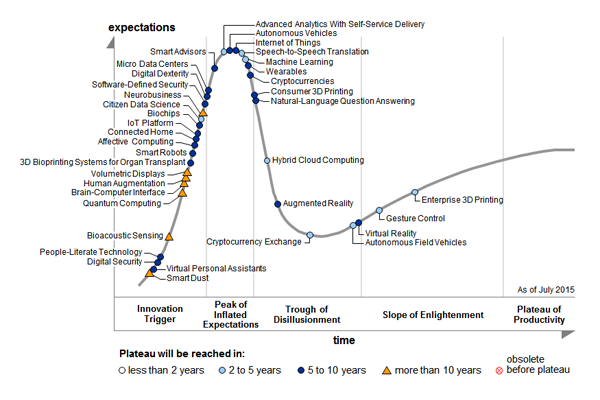
\includegraphics[width=0.9\textwidth]{imagens/gartner.png}
  \label{fig:gartner}
  
  Fonte: \cite{gartner}
\end{figure}

O conceito de casa inteligente � definido por \cite{jiang2004} como "uma resid�ncia incorporando uma rede de comunica��es que conecta servi�os e equipamentos el�tricos, permitindo que eles sejam controlados remotamente, monitorados ou acessados". Esta defini��o explicita o car�ter interativo e automatizado inerente ao conceito, abrindo uma margem muito grande de poss�veis aplica��es de utilidade social. Dentre tais aplica��es, inclui-se prover automa��o residencial e conectividade social \cite{harper2006}, al�m de fornecer um ambiente seguro e monitor�vel a idosos ou deficientes \cite{chan2008}.


\section{Solu��es existentes}\label{sec:solutions}
Acompanhando a populariza��o do conceito de \textit{smart houses}, diversas solu��es e plataformas foram desenvolvidas e lan�adas no mercado. Como exemplos, pode-se citar o Apple HomeKit \cite{homekit}, Wireless Sensor Tags \cite{wsensortags}, WigWag \cite{wigwag} e o Samsung SmartThings \cite{smartthings}.

Todas as solu��es citadas, � exce��o do Apple HomeKit, seguem uma arquitetura similar. Os sensores e atuadores distribu�dos pela resid�ncia s�o conectados a um controlador central , respons�vel por coletar leituras dos sensores e comandar a��es aos atuadores. Al�m disso, este controlador se conecta a um servidor em nuvem, que centraliza o armazenamento de dados e fornece uma interface aos usu�rios para monitorar e definir o estado da resid�ncia.

A solu��o desenvolvida pela Apple baseia-se na utiliza��o dos dispositivos m�veis da empresa para efetuar o monitoramento e controle mencionados. Assim, ela � fortemente dependente do ecossistema Apple para o funcionamento, especialmente pelo fato de o suporte ser dado somente pelo sistema operacional propriet�rio iOS. No entanto, a empresa permite o desenvolvimento de dispositivos de terceiros compat�veis com o HomeKit, atrav�s da disponibiliza��o de um \textit{framework} pr�prio. Os produtos desenvolvidos devem ser certificados pela Apple, processo este envolvendo a obten��o de licen�as e submiss�o a an�lises.

O Wireless Sensor Tags apresenta uma solu��o baseada em um controlador local (\textit{tag manager}) conectado � Internet, disponibilizando diversos sensores compat�veis com o controlador. Basicamente, ele permite a utiliza��o de um aplicativo para monitorar os sensores, definindo alertas de acordo com as leituras obtidas. N�o � mencionado suporte a atuadores, nem a possibilidade de desenvolver dispositivos de terceiros compat�veis com o sistema.

O WigWag tamb�m � uma solu��o baseada em um controlador local (aqui denominado \textit{relay}), podendo operar conectado � nuvem ou n�o. A interface dispon�vel possibilita a defini��o de regras de automa��o, controlando atuadores caso determinadas leituras de sensores forem verificadas. O aspecto mais interessante desta solu��o � a capacidade de integrar dispositivos de terceiros utilizando uma plataforma que se auto-denomina de c�digo  aberto, chamada deviceJS. No entanto, o acesso a esta plataforma se encontra fechado no momento de escrita deste relat�rio.

Por fim, de modo an�logo �s demais, a solu��o SmartThings baseia-se em um controlador local (\textit{hub}), que se conecta a servidores em nuvem pr�prios da Samsung. Esta solu��o destaca-se pelo foco dado � integra��o com dispositivos de terceiros, possuindo a documenta��o mais completa dentre os exemplos analisados. Tal integra��o baseia-se em dois componentes de software b�sicos: \textit{device handlers} e \textit{smart apps}. Os \textit{device handlers} funcionam como \textit{drivers}, sendo executados no controlador local. A fun��o deles � traduzir comandos de alto n�vel do controlador (e.g., ligar a luz) para sinais de controle espec�ficos do dispositivo. Os \textit{smart apps}, por sua vez, adicionam a parte de intelig�ncia do sistema, permitindo a cria��o de regras de automa��o de modo similar ao WigWag. A empresa disponibiliza aos desenvolvedores um ambiente de desenvolvimento completo para implementar os componentes citados.

\section{Motiva��o e Objetivos}\label{sec:goals}
Conforme mencionado, o conceito de \textit{smart houses} tem o potencial de trazer v�rios benef�cios aos usu�rios. Logo, � interessante incentivar o desenvolvimento de sistemas abertos, desvinculando-os de empresas e servi�os espec�ficos e tornando-os mais flex�veis para o usu�rio. Note que, das solu��es apresentadas, nenhuma � genuinamente aberta. As solu��es WigWag e Samsung SmartThings s�o as que mais se aproximam dessa ideologia ao disponibilizar plataformas em c�digo aberto para integrar dispositivos de terceiros, mas ainda possuem protocolos de comunica��o fechados (ao menos n�o documentados) e s�o dependentes de servidores em nuvem pr�prios.

Al�m disso, a intelig�ncia contida nas \textit{smart houses} � razoavelmente limitada nas solu��es existentes. Conforme apresentado anteriormente, toda a intelig�ncia � provida pelo usu�rio, que configura manualmente regras envolvendo sensores e atuadores. Ou seja, uma casa que se autoconfigurasse ou sugerisse regras ou a��es ao usu�rio teria destaque no mercado, eliminando ainda mais a interven��o do usu�rio e fornecendo ainda assim uma  experi�ncia altamente customizada.

Um �ltimo aspecto a se mencionar � o fato de nenhuma das solu��es estar dispon�vel no mercado brasileiro no momento de escrita deste relat�rio (in�cio de 2016). Os equipamentos do SmartThings, por exemplo, nem sequer s�o enviados ao Brasil, estando, pois, indispon�veis para importa��o. V�-se a necessidade, portanto, do desenvolvimento de uma solu��o nacional para o segmento das \textit{smart houses}.

Assim, pode-se dividir o objetivo do presente projeto nos seguintes itens:
\begin{enumerate}[\quad (i)]
	\item Projetar e implementar um \textbf{protocolo aberto de comunica��o em n�vel de aplica��o} para ser utilizada em uma rede de sensores sem fio voltada � automa��o residencial, e
	\item Projetar e implementar um \textbf{algoritmo de aprendizagem de m�quina ou minera��o de dados} de modo a prover automa��o residencial.
\end{enumerate}

%TODO Definir o escopo do projeto


\chapter{Conclus�es}\label{chp:conclusion}

\bibliography{referencias}

\appendix

\chapter{Demonstra��o do Lema da Bifurca��o}\label{app:apendiceA}

\end{document}
